
\section{\textcolor{orange}{Some UQ problems and components}}
\begin{frame}
	\frametitle{Two types of UQ problem}
	\framesubtitle{} % Optional subtitle
        \begin{figure}
            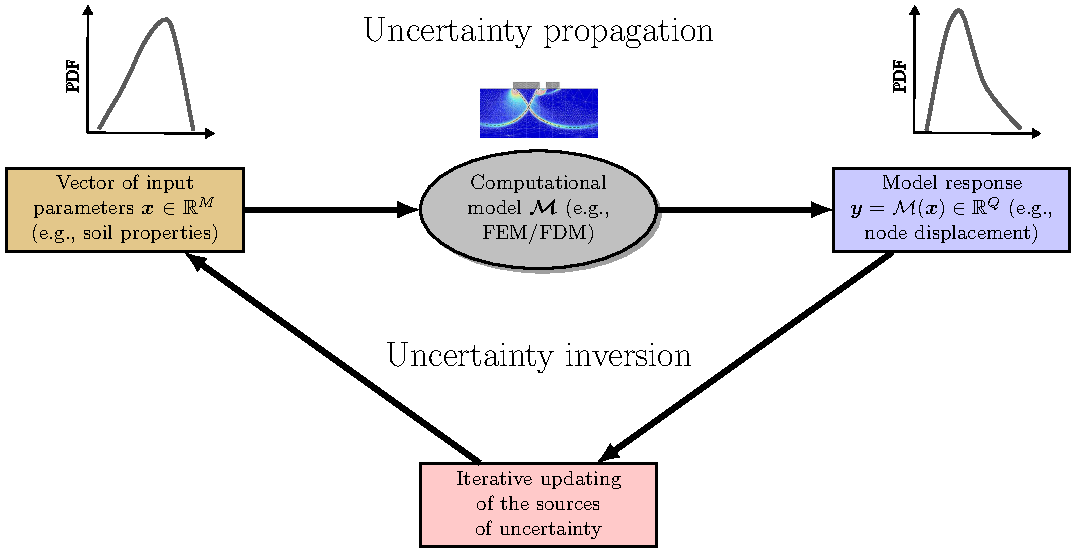
\includegraphics[scale=0.7]{figures/figure-UQ_steps.pdf}
        \end{figure}
\end{frame}

%------------------------------------------------

\subsection{Computational model}
\begin{frame}
	\frametitle{Component one: computational model}
	\framesubtitle{} % Optional subtitle
\begin{definition}
  A computational model should contain:
    \begin{itemize}
        \item a \alert{mathematical description} of the physics 
        \item may be seen as a \alert{black box} to compute the QoI
    \end{itemize}
\end{definition}
\only<1>{
        \begin{figure}            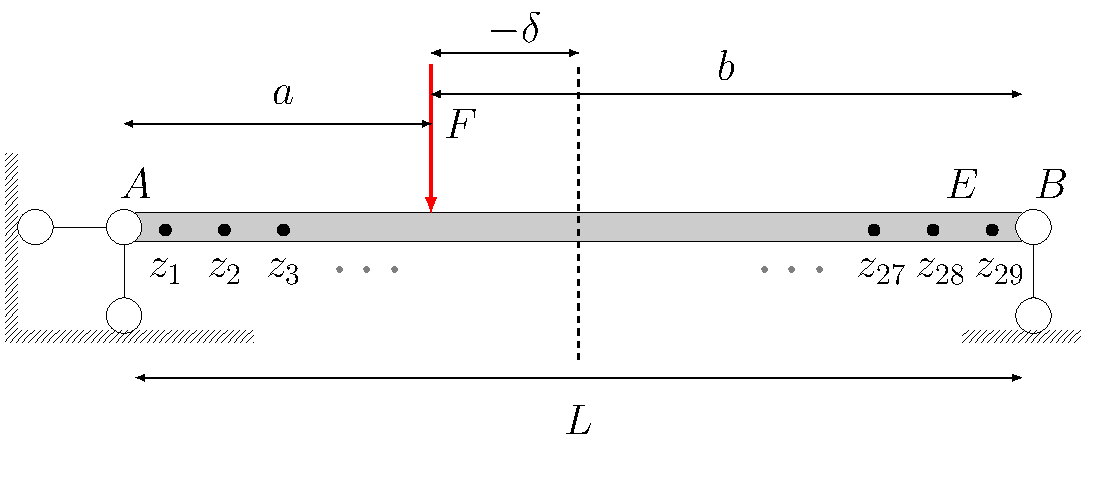
\includegraphics[scale=0.4]{figures/figure-beam.pdf}
        \end{figure}          
        \begin{equation}
                    y = \left\{\begin{matrix}
        \frac{F b  x  [(L^2 - b^2) - x^2]}{6LEI}  \ x \le a
         \\
         \frac{F b  [\frac{L}{b} (x - a)^3 + (L^2 - b^2)]}{6LEI} \ x> a
        \end{matrix}\right.
        \end{equation}
        }


\only<2>{
KJHH model in excavation in predict the deflection \cite{hsein2013}: 
\begin{equation}
\begin{aligned}
    \delta_{hm}(mm) = &a_0 + a_{1}X_1+ a_{2}X_2+ a_{3}X_3+ a_{4}X_4+ a_{5}X_5 + \\
    & a_{6}X_{1}X_{2}+ a_{7}X_{1}X_{3} + a_{8}X_{1}X_{5}
\end{aligned}
\end{equation}
where $X_1$ is the excavation depth, $X_2$ is $EI/\gamma_{w}h_{avg}^{4}$ support stiffness, ...
}


\only<3>{
A model in predict peak resistance\cite{li2018}:

\begin{figure}
    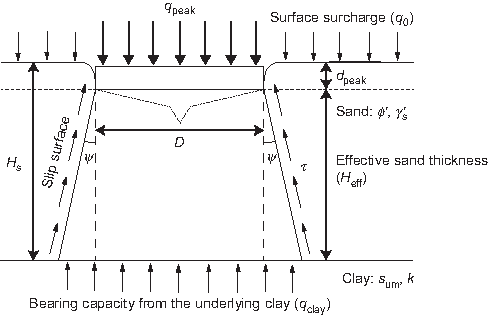
\includegraphics[scale=0.9]{figures/figure-qpeak.pdf}
\end{figure}  
}

\only<4>{
Numerical methods:
\begin{itemize}
    \item Finite element method
    \item Finite difference method
    \item $\cdots$
\end{itemize}
}
\end{frame}

%------------------------------------------------------------------------------------------------------------------------
\subsection{Probabilistic input parameters}
\begin{frame}
	\frametitle{Component two: probabilistic models of input parameters:}

 \begin{block}{No data exist:}
\begin{itemize}
    \item \alert{expert judgment} for selecting the input PDF's
    \item literature, data bases (e.g., on material properties)
    \item maximum entropy principle
\end{itemize}
 \end{block}

\begin{block}{Input data exist:}
\begin{itemize}
    \item classical statistical inference
    \item \alert{Bayesian statistics} when data is scarce but there is some prior information
\end{itemize}
 \end{block}

 \begin{block}{Data on output quantities:}
\begin{itemize}
    \item \alert{inverse} probabilistic methods and \alert{Bayesian updating} techniques 
\end{itemize}
 \end{block}
 
 \end{frame}
 
 %-----------------------------------------------------------------------------------
\subsection{Propagation based on Monte Carlo}
\begin{frame}
	\frametitle{Component three: principles of uncertainty propagation:}

\only<1>{
\begin{block}{Goal}
    estimate the uncertainty/variability of the \textit{QoI} $\boldsymbol{Y} = \mathcal{M}(\boldsymbol{X})$ due to the uncertainty $f_{\boldsymbol{X}}$
\end{block}

\begin{columns}
    \column{0.7\textwidth}
    \begin{itemize}
    \setlength\itemsep{0.5cm}
        \item \alert{Output statistics}, i.e., mean, standard deviation. etc.
        \begin{equation*}
            \mu_{\boldsymbol{Y}} = \mathbb{E}_{\boldsymbol{X}}
[\mathcal{M}(\boldsymbol{X}) ]
        \end{equation*}
        \begin{equation*}
\sigma^2_{\boldsymbol{Y}} = \mathbb{E}_{\boldsymbol{X}}
[(\mathcal{M}(\boldsymbol{X}) - \mu_{\boldsymbol{Y}})^2]
        \end{equation*}

      \item \alert{Distribution} of the QoI

        \item \alert{Probability} of exceeding an admissible threshold $y_{adm}$
       \begin{equation*}
            P_{f} = \mathbb{P}(\boldsymbol{Y} \ge y_{adm})
        \end{equation*}
 
    \end{itemize}
    
    \column{0.3\textwidth}
    \begin{figure}
        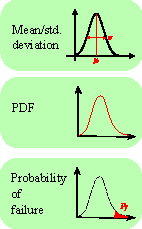
\includegraphics[scale=1.4]{figures/figure-UQpropagation.pdf}
    \end{figure}    
\end{columns}


}
 \end{frame}
 %-----------------------------------------------------------------------------------
 \begin{frame}
 \frametitle{Uncertainty propagation based on Monte Carlo}
 \begin{block}{Principle}
    Reproduce numerically the variability of the model parameters using a random number generator 
 \end{block}

\begin{figure}
    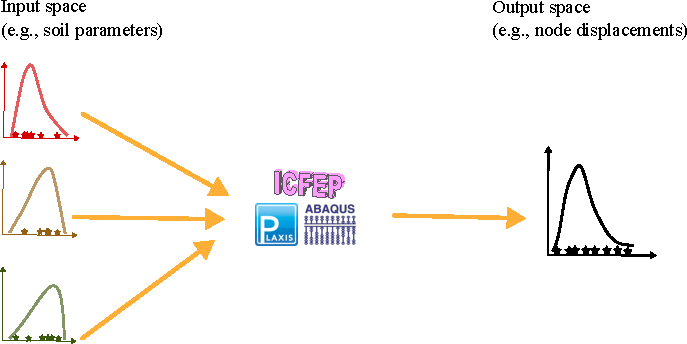
\includegraphics[scale=0.9]{figures/figure-UQ_propagation_MC.pdf}
\end{figure}


 \end{frame}
 %---------------------------------------------------------------------------------------------------
\begin{frame}
\frametitle{Uncertainty propagation based on Monte Carlo}
\framesubtitle{Pros and cons based on Monte Carlo:}

\begin{columns}
    \column{0.5\textwidth}
    PROS:
    \begin{itemize}
        \item \textcolor{red}{Universal methods:} only rely upon simulating random sampling and repeated computational model
        \item Suited to \textcolor{red}{HPC}
        \item Sound statistical foundations: convergence when $N_{MCS} \rightarrow \infty$
    \end{itemize}
    CONS:
    \begin{itemize}
        \item \textcolor{red}{Statistical uncertainty}: results are not exactly reproducible
        \item \textcolor{red}{Low efficiency:} convergence rate $\propto n^{-1/2}$
    \end{itemize}
    \column{0.5\textwidth}
    

\begin{example}{An example}
      To compute $P_{f} = 0.001$ is to be computed:
    \begin{itemize}
        \item At least 1,000 samples are needed in order to observe one single failure
        \item About 100 times more (i.e., 100,000 samples) are required to have a $\pm 10\%$ accuracy
    \end{itemize}  
\end{example}

\end{columns}

\end{frame}
%---------------------------------------------------------------------------------------------------
\subsection{Surrogate model}
\begin{frame}
\frametitle{Surrogate models for uncertainty quantification}
\begin{definition}
A \alert{surrogate model} $\tilde{\mathcal{M}}$ is an approximation of the original computational model $\mathcal{M}$ with the following features:  
\end{definition}
\begin{itemize}
    \item It is built from a \alert{limited} set of runs of the original model $\mathcal{M}$ called the \alert{experimental design} $\mathcal{X} = \{\boldsymbol{x}^{(i))},i=1,\cdots,N\}$
    \item It assume some regularity of the model $\mathcal{M}$ and some general functional shape
\end{itemize}
\begin{table}
\small
\begin{tabular}{lll}
\hline
Name                              & \multicolumn{1}{c}{Shape} & \multicolumn{1}{c}{Parameters} \\ \hline
\alert{Polynomial chaos expansions}       &                           $\tilde{\mathcal{M}}(\boldsymbol{x})
=
\sum_{\boldsymbol{\alpha} \in \mathcal{A} } 
\boldsymbol{y_{\alpha}} \Psi_{\boldsymbol{\alpha}} (\boldsymbol{x})$&                                $\boldsymbol{y_{\alpha}}$\\
Low-rank tensor approximations    &                           $\tilde{\mathcal{M}}(\boldsymbol{x})
=
\sum_{l=1}^{R} b_{l}
\left ( 
\prod_{i=1}^{M}  v_{l}^{i}x_{i}
 \right ) 
$&                                $b_{l}, \  z_{k,l}^{i}$\\
Kriging (a.k.a Gaussian processs) &                           $\tilde{\mathcal{M}}(\boldsymbol{x})
=
\boldsymbol{\beta}^{T} \cdot \boldsymbol{f}(\boldsymbol{x})
 + Z(\boldsymbol{x},\omega)$&                                $\boldsymbol{\beta}, \ \sigma_{Z}^{2}, \  \boldsymbol{\theta}$\\
Support vector machines           &                           $\tilde{\mathcal{M}}(\boldsymbol{x})
=
\sum_{i=1}^{m}
a_{i} K(\boldsymbol{x}_{i},\boldsymbol{x}) 
+b$&                                $\boldsymbol{a}, \ b$\\
Neural networks                   &                           $\tilde{\mathcal{M}}(\boldsymbol{x})
=
f_{n}\left ( 
\cdots f_{2}(
b_{2} + f_{1}(
b_{1} + \boldsymbol{w}_{1} \cdot \boldsymbol{x}
)
\cdot \boldsymbol{w}_{2}
)
\right ) $&                                $\boldsymbol{w}, \ \boldsymbol{b}$\\ \hline
\end{tabular}
\end{table}
\end{frame}


%---------------------------------------------------------------------------------------------------
\begin{frame}
\frametitle{Advantages and challenges of a surrogate}
\begin{block}{Usage}
\centering
$\mathcal{M}(\boldsymbol{x})  \ \ \ \ \approx  \ \ \ \ \tilde{\mathcal{M}}(\boldsymbol{x})$\\
\alert{Hours to run}  \ \ \ \ \ \ \textcolor{green}{seconds to run}
\end{block}

\begin{columns}
    \column{0.5\textwidth}
    \begin{block}{Advantages:}
    \begin{itemize}
        \item \alert{Non-intrusive methods}: Only based on the input-output of the computational model. such as MCS
    \end{itemize}
        
    \end{block}

    \begin{block}{Challenges:}
    \begin{itemize}
        \item Need for a rigorous validation (\alert{overfitting} or \alert{underfitting})
        \item \alert{Not free}: Require too many EoD $\mathcal{X}$ if based on MCS-\alert{\textit{curse of dimensionality}}
        
    \end{itemize}
        
    \end{block}  
    \column{0.5\textwidth}  
    \begin{block}{Need for active learning} \animategraphics[loop,width=7.7cm]{1}{figures-gif/GP-activelearning/GP-}{1}{7}         
    \end{block}
    
    
\end{columns}


\end{frame}


%-------------------------------------------------------------------------------------------------

\begin{frame}
\begin{block}{A flowchart for active learning}
\begin{figure}          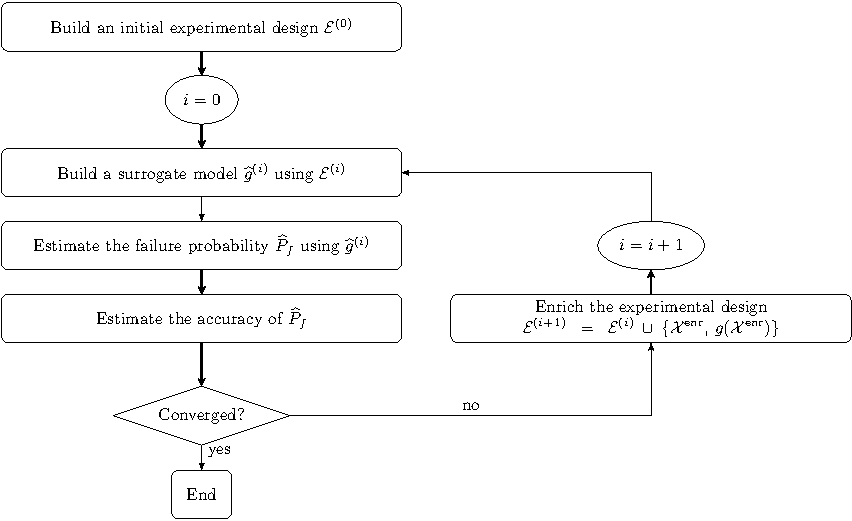
\includegraphics[scale=0.7]{figures/figure-activelearning.pdf}   
\caption{Active learning workflow \cite{moustapha2022}}
\end{figure}  
\end{block}    
\end{frame}
%--------------------------------------------------------------------------------------------
\subsection{sensitivity analysis}
\begin{frame}
\frametitle{Sensitivity analysis}
\begin{block}{Goal:}
Determine what are the input parameters whose uncertainty explains the variability of the QoI    
\end{block}

\begin{columns}
    \column{0.6\textwidth}
    \begin{itemize}
        \item detect input parameters whose uncertainty has \alert{no impact} on the output variability
        \item detect input parameters which allow one to best \alert{decrease the output variability} when set to a deterministic value
        \item detect interactions between paramters
    \end{itemize}
    \column{0.4\textwidth}
\begin{figure}          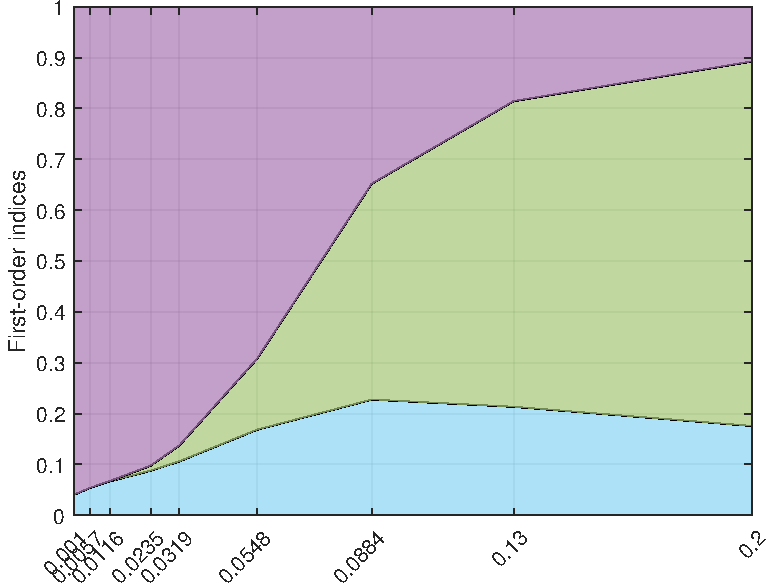
\includegraphics[scale=0.45]{figures/figure-Sobol.pdf}
\end{figure} 
\end{columns}

\end{frame}
%----------------------------------------------------------------------------------------
\begin{frame}
\frametitle{Sobol's indice} 
\begin{block}{Total variance:}
\begin{equation*}
D\equiv \text{Var}[\mathcal{M}(\boldsymbol{X}) ]
= \text{Var}[\sum_{u \subset \{1,\cdots,M\}} \mathcal{M}_{u}(\boldsymbol{X}_{u}) ]
= \sum_{u \subset \{1,\cdots,M\}} \text{Var}[\mathcal{M}_{u}(\boldsymbol{X}_{u}) ] 
\end{equation*}    
\end{block}

\begin{itemize}
    \item Sobol's indice:
    \begin{equation*}
S_u   \overset{\mathrm{def}}{=} \frac{\text{Var}[\mathcal{M}_{u}(\boldsymbol{X}_{u}) ] }{D} 
    \end{equation*}

    \item First-order Sobol's indice:
     \begin{equation*}
S_i = \frac{D_i}{D} = \frac{\text{Var}[\mathcal{M}_{i}(\boldsymbol{X}_{i}) ] }{D}
    \end{equation*}
    Quantify the effect of each input parameter \alert{separately}

    \item Total Sobol's indice:
    \begin{equation*}
S_{i}^{T} \overset{\mathrm{def}}{=}  
\sum_{u \supset i} S_u
    \end{equation*}
    Quantify the \alert{total effect} of $x_{i}$, including \alert{interactions} with other variables

\item 
    
\end{itemize}
\end{frame}